
\documentclass[bsc,frontabs,twoside,singlespacing,parskip,deptreport]{infthesis}
\usepackage{eurosym}
\usepackage{graphicx}
\usepackage{hyperref}
\hypersetup{unicode=true,
			colorlinks=true,
			linkcolor=black,
			urlcolor=cyan,
            pdfborder={0 0 0},
            breaklinks=true}
\urlstyle{same}
\providecommand{\tightlist}{%
  \setlength{\itemsep}{0pt}\setlength{\parskip}{0pt}}

\begin{document}

\title{RegEx Search \& Replace Extension for Chrome and Firefox}

\author{Dalimil Hajek}

\course{Computer Science}
\project{BSc Hons Project Report}
\date{\today}

\abstract{
The aim of this project was to build a browser extension to allow users to search and replace text with regular expressions in editable text input fields of web pages.

After evaluating existing extensions that were unsuccessfully attempting to implement this functionality, the new extension has been carefully designed, developed, and finally successfully released for Chrome and Firefox browsers.

In addition to the future-rich search and replace function, this plugin also adds the ability to save favorite patterns, store search history, or predefine text templates that can be inserted into the editable area of a page.

The software followed an iterative development process, where user feedback was collected via several means, including Google Analytics, which was used to track user interaction, and a support website used to collect user feedback comments.

After the initial release, about twenty updates have been subsequently released over the span of a few months. This iteration was further supported by automated tests of several kinds.

The extension has received excellent reviews and at the time of writing has over 3000 weekly users (users from both browsers combined).
}

\maketitle

\section*{Acknowledgements}
Thanks to
\begin{itemize}
\item
  Boris Grot - for supervising the whole project, and making important feature suggestions leading up to the first official releases of the extension on the Chrome and Firefox web stores
\item
  Michael O'Boyle - for making suggestions, especially regarding Google Analytics
\item
  Christoph Metze - for finding several important bugs that subsequently led to releases \texttt{1.3.2}, \texttt{1.3.3}, and \texttt{1.3.4}
\item
  Daniel Tomberlin - for pointing out a use case when trying to search across multiple single-line inputs, and for updating his web store rating and review after I implemented it in \texttt{1.3.6}
\item
  GitHub user \href{https://github.com/MarkRH}{MarkRH} - for finding a bug that was later fixed in \texttt{1.1.3}
\item
  StackOverflow user \href{https://stackoverflow.com/users/3959875/woxxom}{wOxxOm} - for suggesting \texttt{Document.execCommand} API that I used to fix issues with templates in \texttt{1.2.0}
\end{itemize}

And also thanks to all those people who submitted user feedback or
reviews.

\standarddeclaration

\tableofcontents
\listoffigures

\chapter{Introduction} % should be about 5 pages
Modern web browsers allow users to find text in a web page, but when it comes to editable text areas that are often used on blogging platforms, online forums, social media, and email web clients, as a form of user input, none of the existing browsers allow users to also replace the found occurrences.
 
The aim of this project was to build an extension that adds this browser functionality. The tool allows users to find and replace text in editable text input fields of web pages, and includes a large set of features and search options, including regular expression support and occurrence highlighting.

\section{Motivation}
Search and replace functionality can be extremely useful when composing long emails, writing posts on social media, online forums, or blogging platforms, as well as in any email web clients. 

The most frequent use cases are:
\begin{itemize}
\item Fixing a typographical error -- A word or a phrase may have been used several times with the wrong spelling. This can reoccur several times in a forum post or an email, and it would be convenient to replace everything at once.

This also includes fixing unreadable characters in blog entries such as {\it \^{A}\euro\r{?}}, due to a change in encoding or some unintended text handling.

\item Normalizing incorrectly formatted text -- Regular expressions can be used to detect formatting errors such as multiple spaces before a period, missing upper-case letter, various metric unit formatting errors, and similar. Search and replace extension supporting regular expressions can quickly find and fix these.

\item Renaming a phrase -- Often a word or a phrase that occurs several times throughout a text needs to be corrected or substituted (perhaps using a synonym or a wording that sounds better)
\end{itemize}

Without having a browser extension for search and replace, one could imagine a solution where all text is copied and pasted into an advanced text editor, fixed using the built-in search and replace function, and copied back into the web page input field.

In addition to being a lengthy and time consuming process, this method would in many cases lose all text formatting, because more advanced editable text elements on the web may contain images, emojis, and text containing many formatting tags, which would not be preserved during the copy-pasting.

Additional motivation behind the development of this project was to add search-and-replace related features that are missing even from the more advanced text editors. One of them is storing the search history, and also being able to save favorite search patterns, that can later be quickly accessed. Both of these would save time and increase user productivity.

\section{Existing Extensions}
Web browsers support standard search functionality for any text on a page but no browsers have the find \& replace functionality. Users have asked for this feature on Google Chrome forums\footnote{Google Chrome Forum link: \href{https://productforums.google.com/forum/\#!topic/chrome/Y4UORlpdYfo}{https://productforums.google.com/forum/\#!topic/chrome/Y4UORlpdYfo}}, but the decision of browser developers was to leave the implementation of this functionality to potential text-processing web applications, rather than implementing it as a part of the browser.

\begin{figure}[h]
\centering
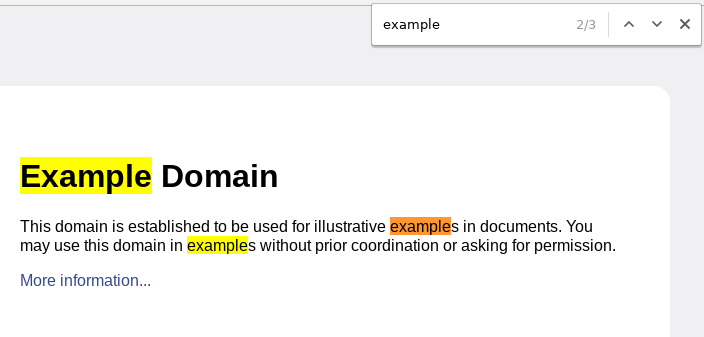
\includegraphics[width=0.6\textwidth]{../docs/browser-find-toolbar/chrome-find.png}
\caption{Google Chrome browser find tool}
\end{figure}

\begin{figure}[h]
\centering
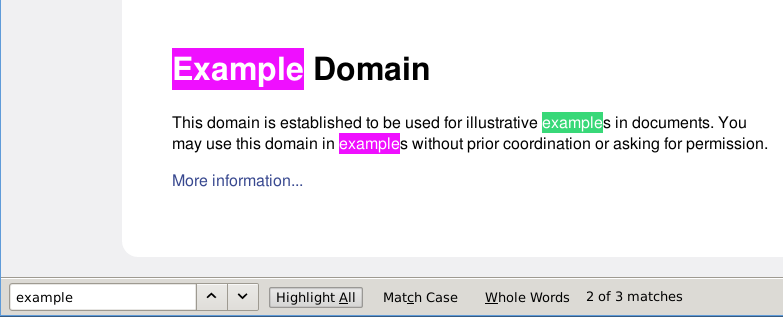
\includegraphics[width=0.6\textwidth]{../docs/browser-find-toolbar/firefox-find.png}
\caption{Mozilla Firefox browser find tool}
\end{figure}

There have been several attempts to implement this functionality via an extension. Most of them either don't work, are missing functionality (particularly support for regular expressions), are limited to certain websites, or are counter-intuitive and hard to use in general. 

\subsection{Chrome}

\begin{itemize}
\item
  {\bf Search and Replace}\footnote{\href{https://chrome.google.com/webstore/detail/search-and-replace/bldchfkhmnkoimaciljpilanilmbnofo}{https://chrome.google.com/webstore/detail/search-and-replace/bldchfkhmnkoimaciljpilanilmbnofo}}
  
  \begin{itemize}
  \tightlist
\item
  This is the dominant one with over 52,000 users (as of Dec 2017)
\item
  It has only $3.1/5$ stars and many reviews are complaining it doesn't work or that it destroys other content of the current page
\item
  It has usability issues (control UI is partially hidden) and it doesn't work in many places such as Blogger or Facebook
\item
  This is a very bad and simplistic solution that is mostly broken but benefits from a larger user base because it appeared in the web store in 2013
  \end{itemize}
  
\item
  {\bf Find Replace}\footnote{\href{https://chrome.google.com/webstore/detail/find-replace/cfjmfciolkikfodjfdmdpdmpfbjdofek}{https://chrome.google.com/webstore/detail/find-replace/cfjmfciolkikfodjfdmdpdmpfbjdofek}}
  \begin{itemize}
  \tightlist
\item
  This extension requires copy-pasting your desired text into the provided box (it is plain-text only, so formatting is lost).
\item
  It has almost 1000 users (as of Dec 2017), but it has been around since 2013
\item
  It is unable to perform the search and replace in browser. This is no better than copy pasting text into a text editor and performing the operation there
  \end{itemize}
\item
  \textbf{FindR}\footnote{\href{https://chrome.google.com/webstore/detail/findr/bidnaaogcagbdidehabnjfedabckhdgc}{https://chrome.google.com/webstore/detail/findr/bidnaaogcagbdidehabnjfedabckhdgc}}
  \begin{itemize}
  \tightlist
\item
  It has almost 2000 users and $3.9/5$ stars. It has been in the web store since April 2016.
\item
  This extension is used for replacing any HTML text in the page, rather than text in input fields -- for this purpose it seems to work, but when one tries to use it only for text input fields, things break and the extension stops working (highlighting and match indicator both disappear and replace button stops working)
\item
  It also requires permission to \textit{Read and change all your data on the websites that you visit}, which might be a privacy issue (the extension can read everything even when the user isn't using it)
  \end{itemize}
\item
  \textbf{Easy Replace}\footnote{\href{https://chrome.google.com/webstore/detail/easy-replace/ojoeejfegihohnkjlfoonbnailkohkce}{https://chrome.google.com/webstore/detail/easy-replace/ojoeejfegihohnkjlfoonbnailkohkce}}
  \begin{itemize}
  \tightlist
\item
  It has over 3000 users but only $2.6/5$ stars
\item
  Most of them report it doesn't work because it only focuses on plain-text text areas and completely ignores more advanced editable HTML elements that most sites use these days
  \end{itemize}
\end{itemize}

\subsection{Firefox}

\begin{itemize}
\item
  \textbf{Find and Replace for Firefox}\footnote{\href{https://addons.mozilla.org/en-US/firefox/addon/find-and-replace-for-firefox}{https://addons.mozilla.org/en-US/firefox/addon/find-and-replace-for-firefox}}
  \begin{itemize}
  \tightlist
\item
  Old add-on, not compatible with the latest Firefox 57.
\item
  It has almost 3000 users but only $3.5/5$ stars
\item
  It's not working for most users, has almost no options (no RegEx, no highlighting, etc.)
\item
  It was last updated in 2012 and is not maintained
  \end{itemize}
\item
  \textbf{FoxReplace}\footnote{\href{https://addons.mozilla.org/en-US/firefox/addon/foxreplace/}{https://addons.mozilla.org/en-US/firefox/addon/foxreplace/}}
  \begin{itemize}
  \tightlist
\item
  This extension provides different functionality -- it asks the user to predefine a list of substitutions and then it automatically applies them globally across the text in newly loaded web pages
\item
  FoxReplace has over 7000 users (Dec 2017) but targets a different audience
  \end{itemize}
\end{itemize}

\subsection{Other Browsers}
Supporting more browsers add extra work, so it only makes sense if these browsers represent a significant portion of the market. The usage share of browsers is measured by various methods and is often quite inaccurate (see \cite{W1}). Approximate values for usage share for desktop browsers are (taken from \cite{A1}): Chrome 65\%, Firefox 12\%, IE 8\%, Safari 6\%, Edge 4\%.

This project focused on Chrome and Firefox, which together represent a large portion of the overall market, and which both mostly follow the same Extension API (there are only a few differences \cite{M5} so we didn't need to have separate code-bases).

Safari, although widely used by Mac users, has its own extension API and is in general much more involved as it requires dealing with Apple's developer libraries and licenses, so we decided not to develop an extension for this browser.


%The Introduction chapter should always provide a 'roadmap' to the report. Of course it should provide an introduction to the problem being considered, but it should also give some details of what you did - do not leave this to the conclusion. You should give forward references into the rest of the report - e.g., "In Chapter 2 how algorithms and heuristics are used to deal with approximate counting are discussed", "The design of the system is presented in Chapter 4", "In Chapter 3 the reasons for choosing to focus on the bounded-degree case of this problem are explained". 

% make sure you point out what was involved in solving certain problems; this can help a non-expert judge the work involved. For instance: "The interpolation algorithm was implemented in C directly, rather than using the routines in Matlab". "In order to develop a user interface appropriate for the educational system, 4 prototypes were tested on 50 students". 

% Use passive voice: A and B were used. instead of I used A and B


\chapter{Background}
A browser extension is a bundled collection of files - HTML, CSS, JavaScript, images and other assets, that together add functionality to the browser. They have access to the standard DOM API (same as a regular website) but in addition to that they can access the WebExtensions API, which is provided by the browser. At the time of writing, the WebExtensions API is to a large extent (only with slight deviations in implementations) supported by Mozilla Firefox, Google Chrome, Microsoft Edge, and Opera browsers (see detailed explanation in \cite{C1}, \cite{C2}, \cite{M6} and \cite{M7}).

A typical extension consists of a background page, which holds the main logic of the extension and has full access to the APIs, pop-up widget, which presents the extension's user interface, and one or more content scripts, which are pieces of JavaScript code that are injected into the current web page so that we can interact with its content.

After installing a browser extension in Chrome or Firefox, a small icon representing the extension is added to the top toolbar. When users click this icon, the extension displays its pop-up widget. The standard way to present an interface to the user is via this widget. One could come up with alternative ways to present extension's UI but this design pattern using a pop-up is the preferred way and something that users expect by default. Since a pop-up widget works well in our scenario, we decided to go with that.

\chapter{Design}

\section{Naming and Search Engine Optimization}
Based on the competition research mentioned in the introduction chapter above, the following extension names already exist: \textit{Easy Replace}, \textit{Search and Replace}, \textit{FindR}, \textit{Find Replace}, \textit{FoxReplace}. Using any of these existing names would be bad for the SEO and discoverability, and would most likely lead to confusions.

At the same time, we want to clearly indicate that the extension is used for input fields and editable content rather than HTML source code.

People are likely to search for browser extensions by typing in the functionality that they need. In our case, that might look something like "find and replace in text input fields extension". Stating the extensions purpose in its title and description should help us do better in search results. Therefore, we avoided any newly-invented words and named it \textit{Find \& Replace for Text Editing}. We are not trying to trademark a new brand name, we are simply trying to match what people might search for, so that's why this name was chosen.

The naming idea was largely successful. In January 2018 (a few months after the first release), the extension ranked 2nd in the Google search results for queries \textit{search and replace in chrome}, and \textit{search and replace browser}, 1st for the query \textit{search and replace in firefox}, 7th for the query \textit{find and replace text}, and 8th for the query \textit{search and replace text}.\footnote{Tested using incognito modes in both Firefox and Chrome, and searching via www.google.co.uk on 25th January 2018}


\begin{figure}[h]
\centering
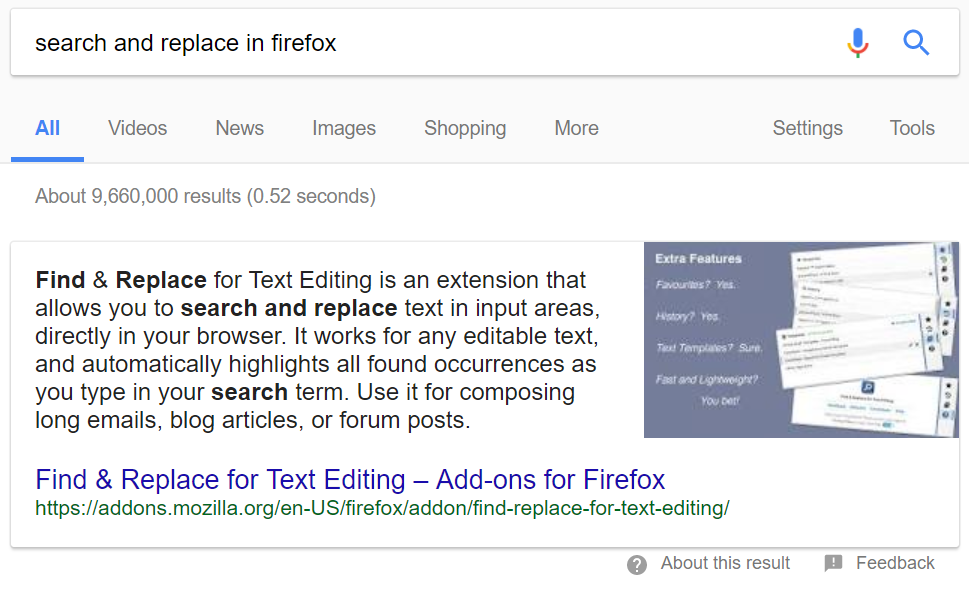
\includegraphics[width=0.7\textwidth]{../docs/search-results.png}
\caption{Google Search Results Ranking}
\end{figure}

\section{User Interface Inspiration}
To some extent, we wanted to follow the current standard of find \& replace toolbars. Many of these can be seen in more advanced text editors. The user interfaces of some of the popular ones were examined and used as an inspiration.

\begin{figure}[hp]
\centering
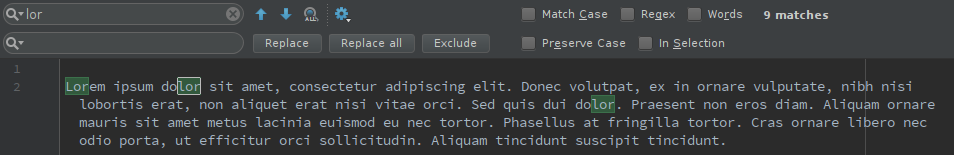
\includegraphics[width=0.9\textwidth]{../docs/editor-find-and-replace/android-studio-find-and-replace.png}
\caption{Android Studio find and replace tool}
\end{figure}

\begin{figure}[hp]
\centering
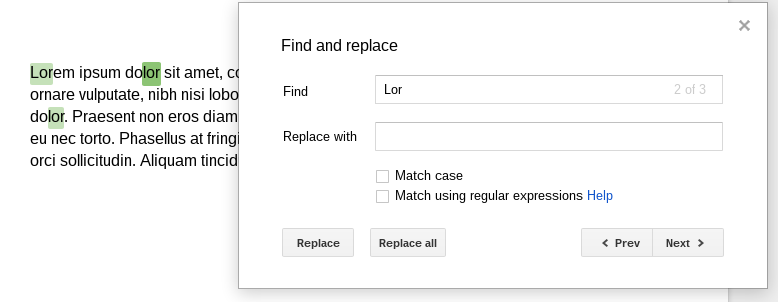
\includegraphics[width=0.9\textwidth]{../docs/editor-find-and-replace/gdocs-find-and-replace.png}
\caption{Google Docs find and replace tool}
\end{figure}

\begin{figure}[hp]
\centering
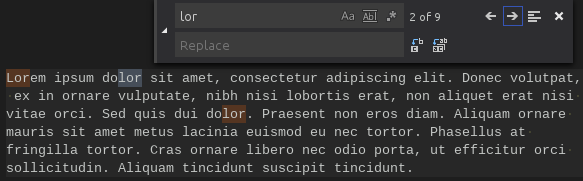
\includegraphics[width=0.9\textwidth]{../docs/editor-find-and-replace/vscode-find-and-replace.png}
\caption{Visual Studio Code find and replace tool}
\end{figure}

\begin{figure}[hp]
\centering
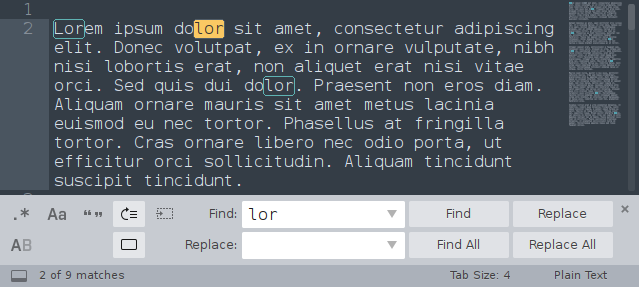
\includegraphics[width=0.9\textwidth]{../docs/editor-find-and-replace/sublime-find-and-replace.png}
\caption{Sublime Text 3 find and replace tool}
\end{figure}

We wanted our extension to follow some of the design patterns that the existing text editors use, so that users are presented with a user interface that they can easily understand and start using quickly.

At the same time, it should not be assumed that average users are familiar with regular expression or more advanced search functions. Therefore, the UI design of some of these editor widgets should only be used as an inspiration - average users are not developers and the number of options in this extension must not feel overwhelming.

\section{UI Components}
To support all the functionality that we specified, the extension widget should have the following UI elements:
\begin{itemize}
\tightlist
\item
  \textit{Find} input field
\item
  \textit{Replace} input field
\item
  \textbf{Action buttons}

  \begin{itemize}
  \tightlist
  \item
    Replace
  \item
    Replace All
  \item
    Find next
  \item
    Find previous
  \item
    Save to favorites
  \item
  	Expand/Collapse advanced search options
  \end{itemize}
\item
  \textbf{Options}

  \begin{itemize}
  \tightlist
  \item
    Match Case (Aa)
  \item
    Whole Word (Ab\textbar{})
  \item
    Use Regex (.*)
  \item
    Limit to Text Selection
  \end{itemize}
\item
  \textit{X of Y} or \textit{No Results} indicator
\item
  Regex groups indicator (for regex search only)
\item
  \textbf{Panel tabs}

  \begin{itemize}
  \item
    Favorites
  \item
    History
  \item
    Templates
  \item
    Help/Info/Feedback
  \end{itemize}
\end{itemize}

We split the user interface layout into two types - simple and advanced. Because displaying all search options in one widget might feel overwhelming for average users, there is a way of switching the search UI to the \textit{advanced} state that includes regex options and helpful previews of matched regex groups etc.

\begin{figure}[h]
\centering
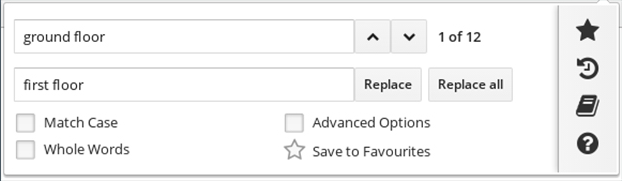
\includegraphics[width=0.95\textwidth]{../graphics/search-widget-simple.png}
\caption{Search widget UI -- simple view}
\end{figure}

\begin{figure}[h]
\centering
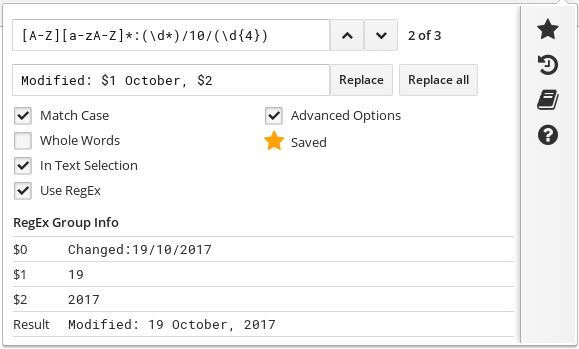
\includegraphics[width=0.95\textwidth]{../graphics/search-widget-advanced.png}
\caption{Search widget UI -- advanced view}
\end{figure}

\section{Why not Material Design}
For the general look and feel, it was decided not to use Google's increasingly popular Material Design \cite{A2} for several reasons. First, Material Design works well when there is a lot of space and all the elements can be spread out. Unfortunately, this extension's user interface is a small widget with very limited space and many condensed components.

Secondly, Material Design likes to add its \textit{ripple effect} to most interactions (such as clicking a button). This looks great for actions that have large impact (e.g. navigating to a new page, or submitting a form), but for our purposes we need something less flashy, as most buttons are going to be pressed very often (\textit{Find next} and \textit{Replace} buttons) and too many effects or animations would present too much distraction for the user.

An extension (a pop-up widget) like ours should, to a large extent, feel like it is part of the browser by perhaps matching some of the user interface styles. We don't want to create an extension that gives users the feeling that it completely doesn't belong because of its wild user interface and flashy styles.

\section{Scope of Search}
Instead of searching in any visible text or simply the HTML source code, we want to limit our search only to elements that contain editable text. There are several ways to create an editable area on web. These are described in \cite{M1} and \cite{P1}.

\subsection{\texttt{\textless{}input\ type="text"\textgreater{}}}

For a short single line of text, HTML
\texttt{\textless{}input\textgreater{}} element is often used. There are
other types of input fields (many new were added with HTML5), such as
date, email, number, tel, time, and similar, but text is the standard
one (see \cite{M2}).

However, due to the short length (20 characters by default), this is not the kind of input that needs the find \& replace functionality on its own. The primary use case of our extension are large multi-line text areas, but we also include the short single-line input kind to allow users to search and replace text in a page across many single-line inputs simultaneously.

\subsection{\texttt{\textless{}textarea\textgreater{}\textless{}/textarea\textgreater{}}}

Multi-line plain-text input space (see \cite{M3}). This should be a common target for find \& replace. It is used by many sites to allow users compose longer pieces of text, one of them is a new post creation process on Reddit.

\subsection{\texttt{\textless{}div\ contenteditable="true"\textgreater{}\textless{}/div\textgreater{}}}

Enabling rich text formatting by allowing HTML tags inside the text
area, \texttt{contenteditable} elements are used in Gmail, Facebook
posts, Facebook Messenger, GitHub editor, Twitter, and many other sites.

Note that \texttt{contenteditable} is a global attribute and is
therefore not limited to \texttt{div} tags (see \cite{M4}).

\subsection{\texttt{contenteditable} tag inside 
\texttt{\textless{}iframe\textgreater{}\textless{}/iframe\textgreater{}}}

Blogger.com is an example of a site that isolates the main
contenteditable area in an iframe. When performing find \& replace we
must consider the scenario where we are dealing with elements inside an \texttt{\textless{}iframe\textgreater{}} on the page.

\subsection{Other DOM}
This extension is not meant to modify (find \& replace) the raw HTML text of the page's source. It is limited to finding occurrences in text areas that are modifiable by users.  

There are certainly sites that might try to avoid all the options discussed above and implement their own text editor functionality. One notable example is Google Docs, which is using static DOM but listen to user's keyboard events to modify it internally in JavaScript. Implementing an online text editor from scratch without using contenteditable or textareas involves a lot of programming work, and such editor should probably include its own find \& replace functionality anyway, which is exactly what Google Docs do.

At the time when the project was first designed, it seemed reasonable to exclude single-line inputs from the scope, as their small editable input space didn't seem suitable for our search and replace functionality. After receiving a lot of user feedback which revealed new use cases, single-line inputs were included in the search scope via an optional checkbox option in the search widget (to ensure backward compatibility and no unexpected behavior for existing users).

\chapter{Implementation}

\section{Search Widget}
To implement the search UI widget, we could simply create DOM elements for all the input components and listen to any changes as the user interacts with the UI. Unfortunately, all input components manage their own state - a better approach would be to store the state of the search parameters in one central place/datastore and have the UI inputs reflect this data. Therefore, we used the React.js library to implement the user interface.

The React library \cite{A3} has become very popular in recent years - one reason is that it enforces the pattern of always reflecting the current application state in the UI. React's internal state is the single source of truth (see React input handling \cite{A4}).

Without it, we would have to manage all the inputs separately and this could create many UI inconsistencies - incorrect update of our internal data might create a state of the application where our search parameters are set to certain values internally but display different state externally via our UI. As we are dealing with a lot of different inputs (many search parameters as well as the simple and advanced modes of the search layout), using React seemed to be a wise choice.

Note that React is only a JavaScript library that allows for a particular way of implementing UI code, but itself doesn't provide any predefined components or styling. The search widget UI was built from scratch without using any existing stylesheets or components.

We set up the project so that we can test the UI widget components in isolation, without creating an actual browser extension and calling the relevant APIs. During development we simply mount our root UI component on a regular website. In production, the same component is mounted in the place of the pop-up widget, which also behaves as a web page.

To also support React's JSX syntax (see \cite{A5}) and newest ECMAScripts language standards, we used Babel \cite{A6} for compiling our JavaScript sources. We used Webpack \cite{A7} to bundle all our source code into a single file, which is obfuscated and small in size. Both of these libraries are widely used and often used in conjunction with React.


\section{Accessibility}

\section{Favorites Panel}
% TODO: explain hashing search state to check if the item is in favourites
\section{History Panel}
\section{Templates Panel}
\section{Help Panel}

%You should always make it clear what was completed, and what was left as future work. If in doubt spell it out: tell us which bits of code you could find already written, which bits you had to do from scratch, which bits were routine, which bits were challenging (and why). 

\chapter{Evaluation}
\section{Distribution and Marketing}
The extension was released on Chrome and Firefox web stores, where users can download it. It was then shared on HackerNews, Quora, Facebook, and several subreddits on Reddit. These sources constituted only a minority of the overall web store visits however, and the major acquisition source remained to be organic Google search (people who specifically search for this extension on Google rather than learning about it via social media or forum posts).

\begin{figure}[h]
\centering
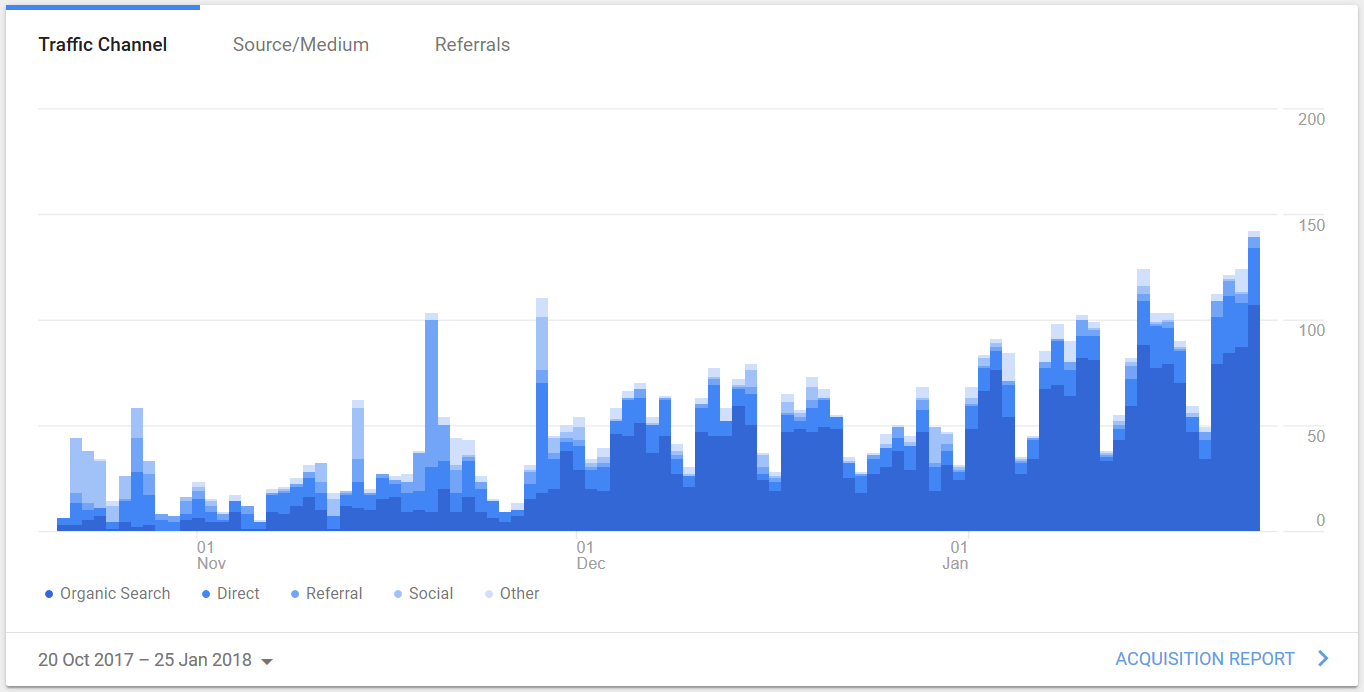
\includegraphics[width=0.99\textwidth]{../docs/user-acquisition.png}
\caption{Chrome web store page - user traffic sources}
\end{figure}

\section{Google Analytics}
In order to collect statistics on how users use our extension and how they interact with different UI elements, we implemented Google Analytics into our extension.

Collecting this data requires us to inform users of the data collection and provide a way for the users to opt-out from collecting these analytics. This might dissuade a small percentage of potential users from installing the extension in the first place, but the belief was that this percentage would me small, which turned out to be true.

\section{Testing}
The Chrome Extension Developer Guides contain a section on debugging \cite{C3} but any standardized extension testing approaches are nonexistent. Due to technology similarities, we can examine how we could test our extension if it was a standard web application.

In such case, we would have several kinds of tests (see \cite{A11}): unit tests testing individual functions, integration tests testing several modules working together, and functional tests testing scenarios using the whole product (in-browser interaction in our case).

\subsection{Unit Tests}
Our content script contains a lot of individual functions that we can test separately. We used \textit{Mocha.js} \cite{A12} for unit testing of individual methods in the content script and search widget. The coverage will be very limited however, because most functions need to interact with the \textit{Document} and \textit{Window} objects, which are supplied by the web browser and will be undefined when running a command line test. We therefore shift our main focus to integration tests and functional tests.

\subsection{Integration Tests}
We would like to test if multiple modules or parts of our code can work well together. We split this into tests for the search widget, and tests for the content script. Testing the extension working as a whole will be addressed in the Functional Tests section.

\section{Support Website}
There are various ways we could collect user-submitted feedback. We could have a website that provides a contact email address or asks users for a feedback message and sends the email automatically. This email inbox could get very cluttered and hard to manage, especially since we want to collect various forms of feedback (e.g. did the user recently uninstall the extension, or are they happy and simply want to propose new features?). 

We decided to proceed with an alternative solution of creating a support website and storing all submitted feedback messages in a database. This database can later be queried and filtered based on various criteria (time of submission, feedback type - general feedback vs complaint after uninstalling, ...), which simplified feedback evaluation.

We created a static landing page website that presents the extension with relevant links to the browser web stores, and also allows users to submit feedback via a simple form.

\begin{figure}[h]
\centering
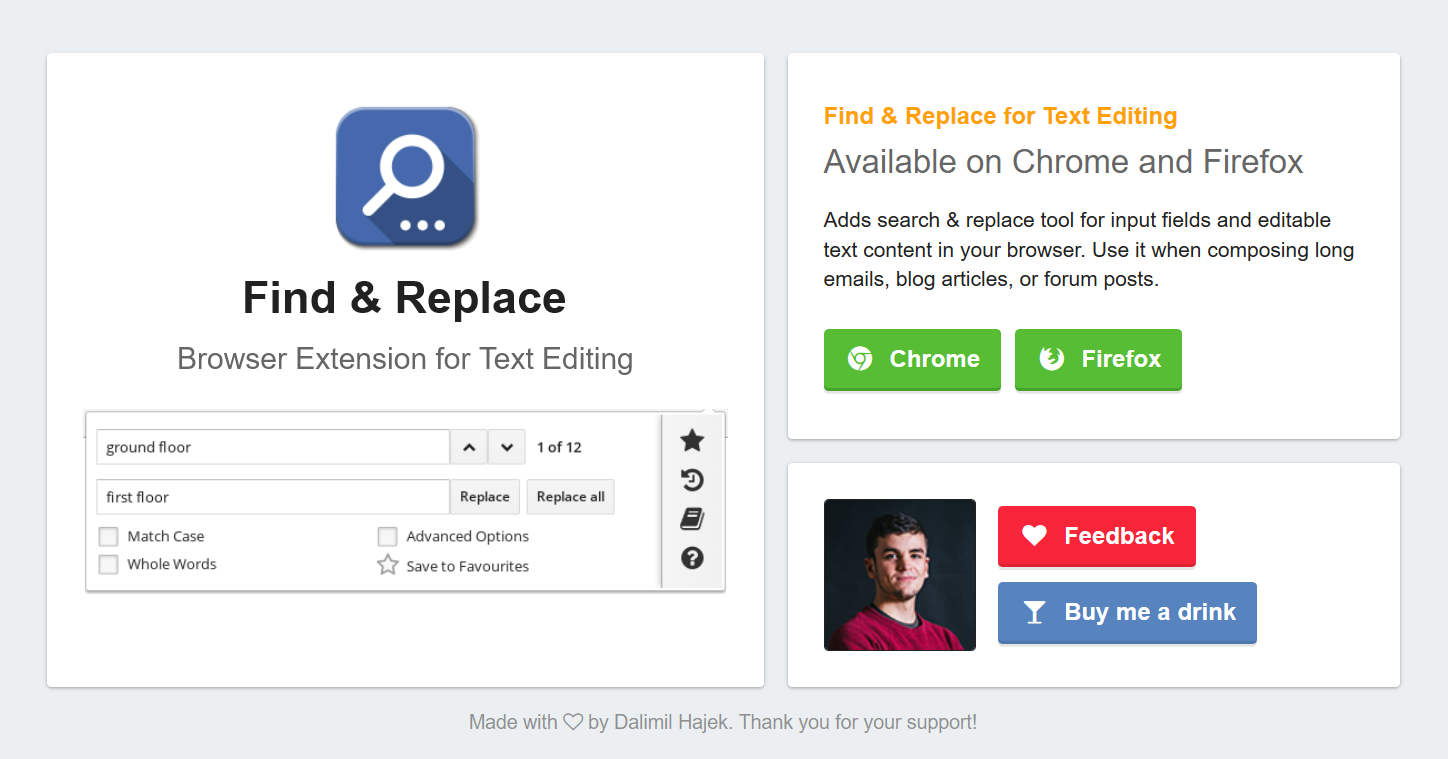
\includegraphics[width=0.99\textwidth]{../graphics/landing-page.png}
\caption{Support website landing page}
\end{figure}

The website was deployed using Firebase Hosting \cite{A8}, which is Google's hosting for deploying static content to its content-delivery network (CDN).

The database used to store the feedback comments is Firebase Realtime Database \cite{A9}, which is a NoSQL cloud database from the same family of Google products. This allowed us to have a secure place to store our data with minimal setup time. It also allowed us to have an optimized static website with only the required JavaScript SDKs without having to implement a complex back-end server.

\section{Iteration}
After the initial web store release we continued to collect feedback from the users, and subsequently kept releasing updates to the extension that were fixing found bugs and issues.

% TODO: insert changelog here

\chapter{Conclusions}
The extension has received excellent reviews and at the time of writing has over 3000 weekly users (users from both browsers combined), $4.7/5$ stars (14 reviews) on the Chrome Web Store and $4.9/5$ stars (7 reviews) on the Firefox Web Store.

\section{Further Work}
Facebook, Quora, and several other sites use contenteditables and keep the text content separately in JavaScript variables. When we insert our highlighting markup, and replace text, their JavaScript immediately restores the previous state (switches back to the original text). We could completely detach their JavaScript listeners, but that stops saving any further changes to the text. This is because the text that is posted is the content of their JavaScript variables, and not the current contenteditable content.

We sought help on StackOverflow, but the only suggestion received was trying \texttt{Document.execCommand} API \cite{A10}, which is a mostly deprecated API that was meant to be replaced by contenteditable. It is currently implemented inconsistently across browsers, and using it to replace a piece of text involves manipulating the active cursor selection programmatically. Even after a lot of testing it proved very unreliable and even the W3C specification currently advises against using it.

Google Docs, Jupyter Notebook, or websites using the CodeMirror plugin, are also currently broken. These web apps don't use textareas or contenteditable to store editable text. Instead they implement their own user input handling and then convert, store, and display everything as raw HTML.

Fixing these sites would mean implementing the search \& replace functionality for any source HTML, which is something that we excluded from our scope from the very beginning and instead decided to limit our extension targets to the standard editable text elements.

Google Docs implement their built-in find \& replace tool anyway. When users try to use the extension on one of the above-mentioned websites that are known to be broken, we spawn a small notification informing the user, and cancel the extension's operation.

\section{Final Word}
Overall, bugs and issues that were found were all fixed in subsequent web store releases of the extension. The issues with the sites mentioned above had no straightforward solutions and were either reaching limits of extension API capabilities or were completely out of scope.

In summary, it makes one feel extremely positive, having developed a tool that is used by thousands of people, and which makes their work faster and more productive every day.

% Bibliography section --- use \cite{P1} with BibTeX
\bibliographystyle{plain}
\bibliography{mybibfile}

\end{document}
